\documentclass[11pt]{article}

\usepackage{graphicx}

\setlength{\textwidth}{160mm}
\setlength{\textheight}{230mm}
\setlength{\topmargin}{-2mm}
\setlength{\oddsidemargin}{0mm}
\setlength{\evensidemargin}{0mm}
\setlength{\parindent}{0mm}
\setlength{\parskip}{\medskipamount}
\setlength{\unitlength}{1mm}


\begin{document}


\section{Registration of INT Wide Field Camera CCD images}

The Wide Field Camera instrument on the Isaac Newton Telescope 
contains four CCD chips, each 2048 x 4096 pixels, 
in roughly the following orientation:
\begin{quote}
\begin{center}
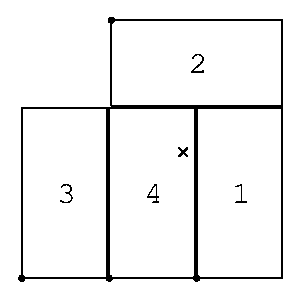
\includegraphics{ideal.ps}
\end{center}
\end{quote}
In order to do accurate astrometry with frames obtained
from this instrument, it is necessary to correct for the 
exact orientation and position of each CCD in relation to
the others, as well as for nonlinear distortions
away from the optical axis of the focal plane introduced by
the optics of the telescope.
The nonlinear distortion is very well modelled by a radial ``pincushion''
transformation, which has the form
\begin{displaymath}
  r^\prime = r ( 1 + D r^2 )
\end{displaymath}

The following transformations take account of both these effects
to map the pixel coordinates $(x_i, y_i)$
of CCD\#$i$ into a new pixel-like coordinate system 
$(x^\prime, y^\prime)$
of uniform scale, which is the same for all four CCDs.
The origin of this coordinate system is at pixel coordinates
$(1778, 3029)$ of CCD\#4, which is taken to be on the optical axis.
At this point, one unit of the new coordinate system is equivalent
to one pixel of the CCD\#4 system, so that the new coordinates 
are almost equivalent to CCD\#4 coordinates (though they diverge
away from the origin thanks to the nonlinear distortion).
Each unit of the new coordinates has the same size, 
which is approximately 0.3334 arcsec.

The corrected coordinates $(x^\prime, y^\prime)$ are obtained from 
each set of pixel coordinates $(x_i, y_i)$
by first translating so that the origin is on the optical
axis, then rotating to the correct angle, 
then correcting for the radial distortion effect:
\begin{eqnarray*}
  x_i^{\rm shift} & = & x_i - X_i \\
  y_i^{\rm shift} & = & y_i - Y_i \\[1ex]
%
  x_i^{\rm rot}   & = & x_i^{\rm shift} \cos \theta_i 
                      - y_i^{\rm shift} \sin \theta_i  \\
  y_i^{\rm rot}   & = & x_i^{\rm shift} \sin \theta_i 
                      + y_i^{\rm shift} \cos \theta_i  \\[1ex]
%
  x^\prime        & = & x_i^{\rm rot} 
                        \left( 1 + D \left[ \left. x_i^{\rm rot} \right.^2 
                                          + \left. y_i^{\rm rot} \right.^2
                                     \right] \right)  \\
  y^\prime        & = & y_i^{\rm rot} 
                        \left( 1 + D \left[ \left. x_i^{\rm rot} \right.^2
                                          + \left. y_i^{\rm rot} \right.^2
                                     \right] \right)
\end{eqnarray*}
Where $(X_i, Y_i)$ are the coordinates of the optical centre of
the instrument in the pixel coordinate system of CCD\#$i$,
$\theta_i$ is the angle at which CCD\#$i$ sits on the focal plane,
and $D$ is the pincushion distortion coefficient.

Values for these coefficients have been obtained by registering
two exposures of the same region of sky, in which the instrument
had been rotated by $180^\circ$ between exposures.
The value of $(X_4, Y_4)$ was taken from the value used 
for the Wide Field Survey data, and $\theta_4$ was chosen to be zero.
The values of the coefficients in these equations are approximately:
\begin{displaymath}
  \begin{array}{c@{\ =\ }r@{\hspace{3em}}c@{\ =\ }r@{\hspace{3em}}c@{\ =\ }r}
     X_1 & -336.74  &  Y_1 & 3039.14  &  \theta_1 &   0.01868^\circ  \\
     X_2 & 3180.68  &  Y_2 & 1729.67  &  \theta_2 & -90.62115^\circ  \\
     X_3 & 3876.73  &  Y_3 & 2996.30  &  \theta_3 &   0.11436^\circ  \\
     X_4 & 1778.00  &  Y_4 & 3029.00  &  \theta_4 &   0.00000^\circ  
  \end{array}
\end{displaymath}
and
\begin{displaymath}
     D = -5.30 \times 10^{-10} {\rm pixel}^{-2}
\end{displaymath}
This value of $D$ corresponds in units of radians to $-20\,3{\rm rad}^{-2}$, 
compared to the value $-259.8\,{\rm rad}^{-2}$
quoted in the ING observer handbook.

These values of the coefficients are thought to be correct to an
accuracy of about 1 pixel $\approx$ 1/3 arcsec.

The following image gives an exaggerated representation of the 
shapes and positions of the CCDs as mapped on to the new coordinate system.
The dots in the corners of the CCDs mark the pixel origin for each CCD
and the ``$\times$'' marks the origin of the unified coordinate system.
\begin{quote}
\begin{center}
\includegraphics{exag4.ps}
\end{center}
\end{quote}

\vspace{\fill}


\begin{flushright}
\it
Mark Taylor \\
24 March 2000
\end{flushright}


\end{document}

% $Id$
